\documentclass{beamer}
\usepackage[utf8]{inputenc}

\usetheme{CambridgeUS}
\usecolortheme{default}
\usepackage{tikz}
\usepackage{caption}
\captionsetup{font=scriptsize,labelfont=normalsize}
\captionsetup[figure]{labelformat=empty}
\captionsetup[table]{labelformat=empty}
\captionsetup[subfigure]{labelformat=empty}
\setbeamertemplate{caption}{\raggedright\insertcaption\par}


\newcommand{\smallindent}{\hphantom{N}}

\usepackage{lmodern}
\usepackage{siunitx}
\usepackage{booktabs}
\usepackage{etoolbox}

\usepackage{amsmath,amssymb}
\usepackage{graphicx}
\usepackage{subcaption}
\usepackage{xcolor,colortbl}

\definecolor{orange}{rgb}{0.8, 0.33, 0.0}
\definecolor{cblue}{rgb}{0.74, 0.83, 0.9}

\setbeamercolor{alerted text}{fg=orange}
\setbeamercolor*{palette primary}{fg = orange}
\setbeamercolor*{palette secondary}{fg = orange}
\setbeamercolor*{palette tertiary}{bg=orange, fg = white}
%\setbeamercolor*{palette quaternary}{bg=orange, fg = green}


\newcommand{\mycomment}[1]{}

%------------------------------------------------------------
%This block of code defines the information to appear in the
%Title page
\title[Master Thesis] %optional
{Advancing Packet-Level Traffic Predictions\\ with Transformers}
\date{\tiny September 1, 2022}
\author[ Siddhant Ray] % (optional)
{Siddhant Ray}

\institute[ETH Zürich] % (optional)
{
  D-ITET \\
  ETH Zürich
}



%\date[September 2022] % (optional)

\titlegraphic{
    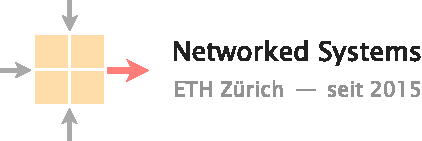
\includegraphics[width=3cm]{figures/nsg_logo.pdf}
    \hspace{2cm}
     
\includegraphics[width=3cm]{figures/eth_logo.pdf}
}

%End of title page configuration block
%------------------------------------------------------------



%------------------------------------------------------------
%The next block of commands puts the table of contents at the 
%beginning of each section and highlights the current section:

%\AtBeginSection[]
%{
%  \begin{frame}
 %   \frametitle{Table of Contents}
 %   \tableofcontents[currentsection]
 % \end{frame}
%}
%------------------------------------------------------------


\begin{document}

%The next statement creates the title page.
\frame{\titlepage}


%---------------------------------------------------------
%This block of code is for the table of contents after
%the title page
%\frametitle{Table of Contents}
%
%end{frame}
%---------------------------------------------------------


\section{Motivation}

\begin{frame}
\frametitle{Machine learning methods we use in networks today}
\pause
\begin{itemize}
    \item<1-> Some data
    \item<1-> Some data++
    \pause
    \item<2-> More data 
     \item<2-> More data++
\end{itemize}
\end{frame}



%---------------------------------------------------------
%Changing visivility of the text
\begin{frame}
\frametitle{Why use Transformers?}
\pause
\begin{itemize}
    \item<1-> Efficient learning with attention mechanism
    \item<1-> Generalizing using large datasets available
    \pause
    \item<2-> State-of-art for sequence learning problems
     \item<2-> Network packet data is a sequence
\end{itemize}
\end{frame}


%---------------------------------------------------------
%Example of the \pause command
\begin{frame}
\frametitle{Transformer's unprecendented successes in generalizing to tasks in NLP and CV}
\pause

BERT: Generalizing to tasks in NLP

\begin{itemize}  
    \item<1-> Sentiment analysis
    \item<1-> Question answering
    \item<1-> Paraphrase detection
\end{itemize}
\pause

Vision Transformer: Generalizing to tasks in CV

\begin{itemize}  
    \item<1-> Image classification
    \item<1-> Object detection
    \item<1-> Image segmentation
\end{itemize}



\end{frame}
%---------------------------------------------------------


\begin{frame}
\frametitle{Our Transformer}

We present the Network Traffic Transformer(NTT):
\pause

\begin{figure}[!hbt]
  \begin{center}
    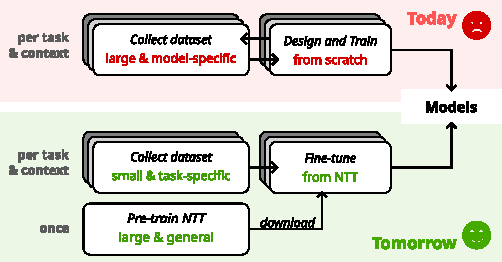
\includegraphics[scale=1]{figures/vision.pdf}
    \caption{Pre-train today, fine-tune and re-use tomorrow}
    \label{fig:vision}
  \end{center}
\end{figure}
    
    
\end{frame}

%---------------------------------------------------------

\section{Design}

%---------------------------------------------------------
%Highlighting text

\begin{frame}
\frametitle{Developing our NTT architecture}
\pause

\begin{figure}[!hbt]
  \begin{center}
    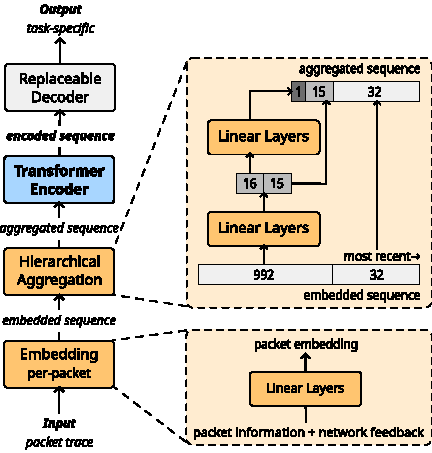
\includegraphics[scale=0.8]{figures/architecture_ntt.pdf}
    \caption{The Network Traffic Transformer (NTT) with
        an embedding layer, % for feature extraction,
        an aggregation layer, and
        a transformer encoder.}
    \label{fig:ntt}
  \end{center}
\end{figure}
\end{frame}

\begin{frame}
\frametitle{Developing our NTT architecture}

Feature selection for NTT's input data:
\pause 
\begin{itemize}
    \item<1-> \alert{Relative timestamp:} To learn sequence order
    \item<1-> \alert{End-to-end delay:} To learn network state information
    \item<1-> \alert{Packet size:} To learn packet state information
\end{itemize}

\end{frame}

\begin{frame}
\frametitle{Developing our NTT architecture}

NNT's learning strategies: 
\pause 
\begin{itemize}
    \item<1-> \alert{Masking delays:} Reconstruct masked values to learn sequences 
    \item<1-> \alert{Variable masking:} Robust learning with multi-positional masks
    \item<1-> \alert{Aggregating inputs:} To learn and scale to larger sequences
\end{itemize}
\end{frame}



\begin{frame}
\frametitle{Pre-training setup}


\begin{figure}[h]
  \begin{center}
    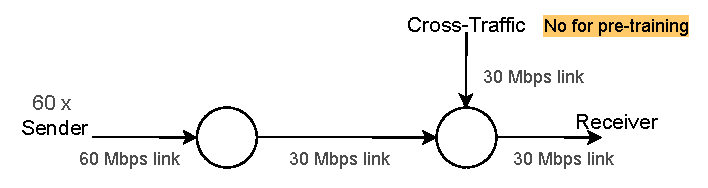
\includegraphics[scale=0.8]{figures/simple_topo.pdf}
    \caption{Initial topology for data generation}
    \label{fig:topo}
  \end{center}
\end{figure}
 
 \pause

\begin{itemize}
    \item<1-> Varied start times across sender application flows
    \item<1-> Ensure to have enough variance in pre-training data dynamics 
    \end{itemize}

\end{frame}

\begin{frame}
\frametitle{Pre-training setup}


\begin{figure}[h]
     
    \captionsetup[subfigure]{justification=centering}
    \begin{subfigure}[h]{0.5\textwidth}
    	\begin{center}
        \centering
        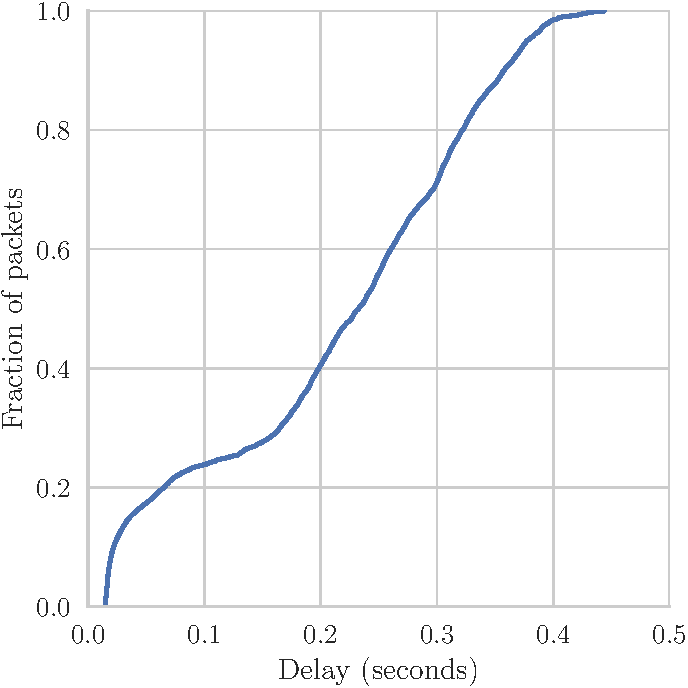
\includegraphics[scale=0.5]{figures/delay.pdf}
        \caption{Delay CDF, single simulation run}
        \end{center}
    \end{subfigure}%
    ~ 
    \begin{subfigure}[h]{0.5\textwidth}
    	\begin{center}
        \centering
        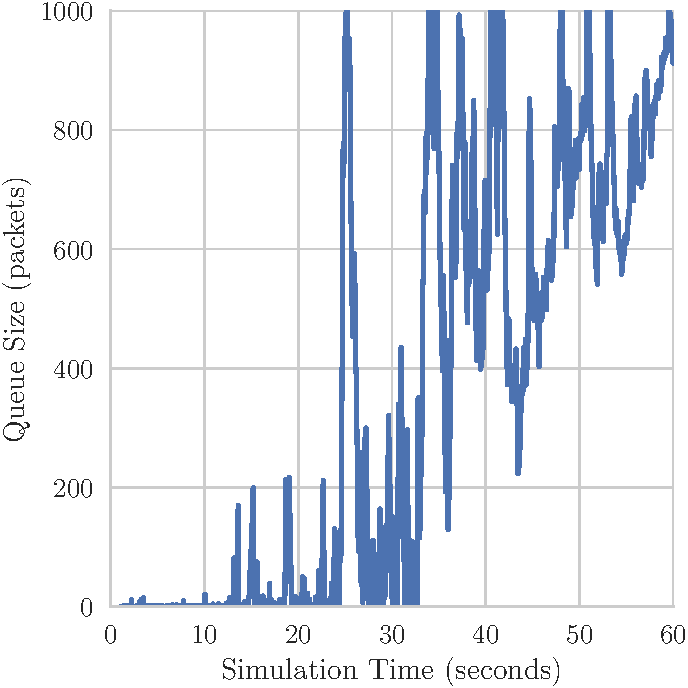
\includegraphics[scale=0.5]{figures/queue_profile_A.pdf}
        \caption{Bottleneck queue profile on the single-path topology}
        \end{center}    
    \end{subfigure}
    \caption{Distribution plots on pre-training data}
    \label{fig:datadist}
    \end{figure}

\end{frame}



%---------------------------------------------------------

\section{Evaluation}

%---------------------------------------------------------
%Two columns
\begin{frame}
\frametitle{Understanding NTT's Performance}


\begin{figure}[h]
  \begin{center}
    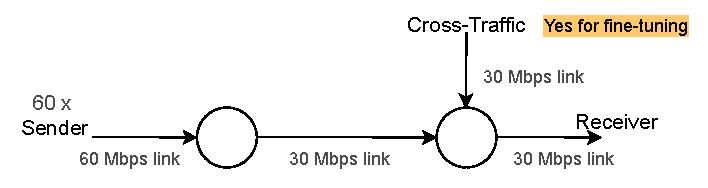
\includegraphics[scale=0.8]{figures/simple_topo_ft.pdf}
    \caption{Fine-tuning data generation, single path topology}
    \label{fig:topo_ft}
  \end{center}
\end{figure}

\pause 

\begin{itemize}
    \item<1-> Two bottleneck dynamics to learn 
    \item<1-> Packet-level fine-tuning task : Predict last delay
    \item<1-> Flow-level fine-tuning task : Predict Message Completion Time (MCT)
    \end{itemize}

\end{frame}


\begin{frame}
\frametitle{Understanding NTT's Performance}


\begin{table}[htbp]
\footnotesize
\centering
\sisetup{detect-weight,mode=text}
% for avoiding siunitx using bold extended
\renewrobustcmd{\bfseries}{\fontseries{b}\selectfont}
\renewrobustcmd{\boldmath}{}
\newrobustcmd{\B}{\bfseries}
\begin{tabular}{ l   c   c  c }
\toprule
\emph{all values $\times10^{-3}$} & Pre-training  & \multicolumn{2}{c}{Fine-tuning} \\
\cmidrule{3-4}
                                                       & {Delay}        & {Delay}                           & {log MCT} \\
\midrule
\em{NTT}                                                 &                &                                   &           \\
    \rowcolor{cblue}
    \smallindent Pre-trained                                 & \B 0.072          & \B 0.097                             & \B 65        \\
    \smallindent From scratch                                & {-}            & 0.313                             & 117       \\
    \noalign{\vskip 1mm}
    \em{Baselines}                                                                                                                 \\
    \smallindent ARMA                                            & 1.800        &  1.180                              &1412 \\
    \smallindent Last observed                               & 0.142          & 0.121                             & 2189      \\
    \smallindent EWMA                                        & 0.259          & 0.211                             & 1147      \\
    \noalign{\vskip 1mm}
    \em{NTT (Ablated)}                                                                                                        \\
    \smallindent No aggregation                              & 0.258          & 0.430                             & 61        \\
    \smallindent Fixed aggregation                           & 0.055          & 0.134                             & 115       \\[0.75mm]

    \smallindent Without packet size                         & 0.001          & 8.688                             & 94        \\
    \smallindent Without delay                               & 15.797         & 10.898                            & 802       \\
     \bottomrule

\end{tabular}
\caption{Mean Squared Error (MSE) for all NTT models and tasks for the single path topology}
\label{eval:table1}
\end{table}
\end{frame}

\begin{frame}
\frametitle{Variable masked pre-training}

Variable masking strategies: For \emph{bi-directional} learning
\pause
\begin{itemize}
    \item<1-> Masking over last 16 delays, no mask over aggregates
    \item<1-> Masking over last 32 delays, no mask over aggregates 
    \pause
    \item<2-> Choose mask over encoded states,  also mask over aggregates
     \item<2-> Choose mask over aggregation levels,  also mask over aggregates
\end{itemize}


\end{frame}

\begin{frame}
\frametitle{Variable masked pre-training}


\begin{figure}[h]
    \centering
    \begin{subfigure}[h]{0.5\textwidth}
        \centering
        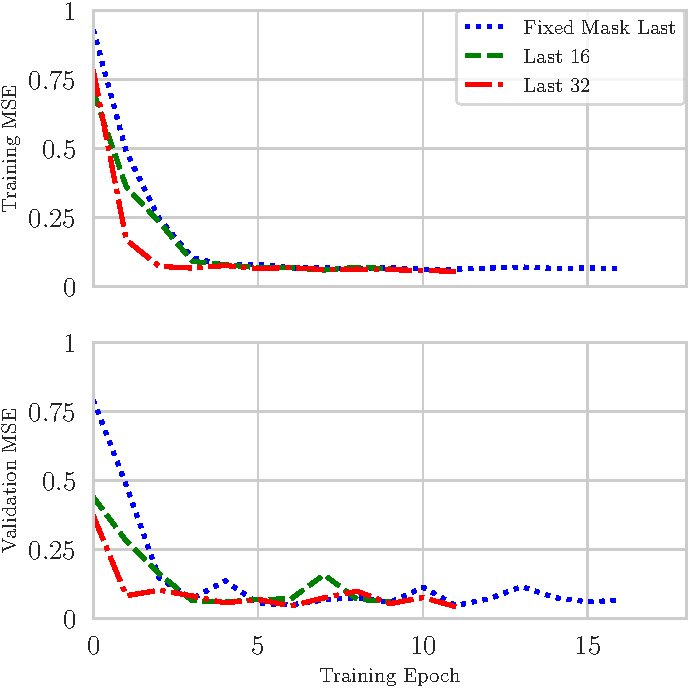
\includegraphics[scale=0.5]{figures/finetune_mct_loss_comparison.pdf}
        \caption{Pre-train with no mask over aggregated delays}
    \end{subfigure}%
    ~ 
    \begin{subfigure}[h]{0.5\textwidth}
        \centering
        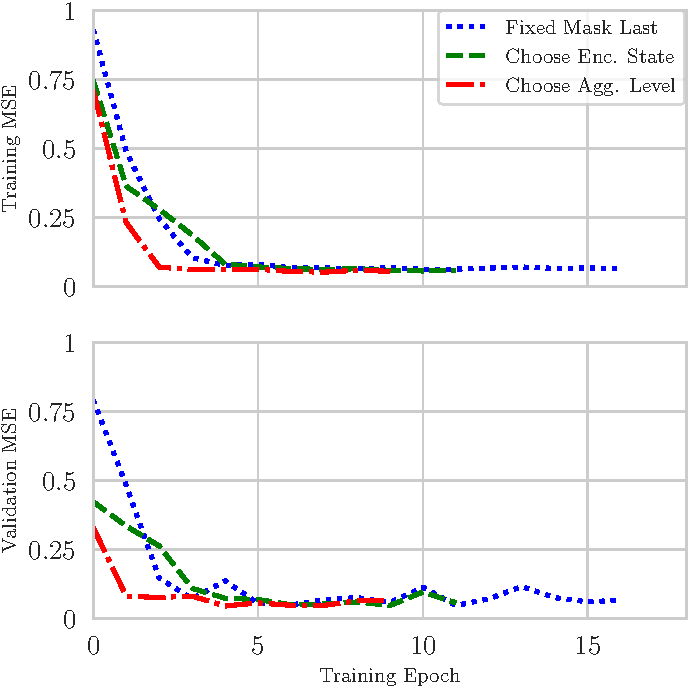
\includegraphics[scale=0.5]{figures/finetune_mct_loss_comparison_agg.pdf}
        \caption{Pre-train with also mask over aggregated delays}
    \end{subfigure}
    \caption{Mean-square error on MCT predictions with different pre-training masks}
    \label{fig:mct_mask}
\end{figure}
\end{frame}

\begin{frame}
\frametitle{NTT on multi-path topologies}


\begin{figure}[h]
  \begin{center}
    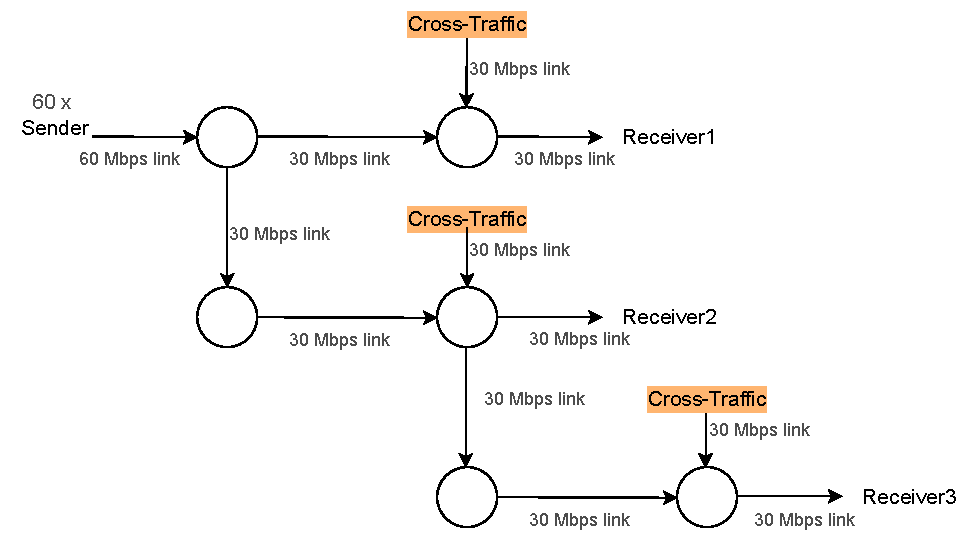
\includegraphics[scale=0.55]{figures/complex_topo.pdf}
    \caption{Fine-tuning data generation on multi-path topology}
    \label{fig:topo_ft_big}
  \end{center}
\end{figure}

\pause 

\begin{itemize}
    \item<1-> Different path delays due to different number of links 
    \item<1-> Receiver ID as additional input feature to distinguish paths
\end{itemize}

\end{frame}

\begin{frame}
\frametitle{NTT on multi-path topologies}


\begin{table}[htbp]
\scriptsize
\centering
\sisetup{detect-weight,mode=text}
% for avoiding siunitx using bold extended
\renewrobustcmd{\bfseries}{\fontseries{b}\selectfont}
\renewrobustcmd{\boldmath}{}
\newrobustcmd{\B}{\bfseries}

\begin{tabular}{ l   c   c  }
\toprule
\emph{Model} &  MSE: Delay Prediction & \# of Epochs    \\
			&		\emph{all values$\times10^{-3}$}  & trained 	\\ 
			

\midrule
\em{NTT}                                                               &       \\      
    \rowcolor{cblue}                                
    \smallindent Pre-trained  +   Fine-tune (full)                                  & \B 0.004   &     \B 5    \\          
    \rowcolor{cblue}        
    \smallindent Pre-trained  +   Fine-tune ($10\%$)                                  & \B 0.035   & \B 12  \\                        
    \smallindent From scratch  + Fine-tune (full)                                       & 5.2    &   10 \\                      
     \smallindent From scratch  + Fine-tune ($10\%$)                                    & 8.2  & 15 \\                          
 \em{Baselines} &       \\  
    \smallindent ARMA  &       					4.2	& - \\  
    \smallindent Last observed &     				11.2	& -  \\  
    \smallindent  	EWMA &     					4.0	& -  \\  
\em{NTT (Ablated)}           &       \\       
     \smallindent Pre-trained  +   Fine-tune (full)  : No Receiver ID                              & 2.8   &     8    \\   
      \smallindent From scratch  + Fine-tune (full) : No Receiver ID                                  & 2.7    & 15  \\         
 
 \bottomrule

\end{tabular}
\caption{Fine-tuning NTT on the multi-path topology}
\label{eval:table5}
\end{table}

\end{frame}






%---------------------------------------------------------

\section{Future}

\begin{frame}
\frametitle{How do we improve the NTT further?}
\pause
\begin{itemize}
    \item<1-> NTT Scaling
    \begin{itemize}
    	\item<1-> Learn additional network features.
	\item<1-> Learn on larger topologies.
    \end{itemize}
    \vspace{0.2cm}
    \pause
    \item<2-> Federated Learning
    \begin{itemize}
    	\item<2-> Share models, not data.
	\item<2->Keep data private.
	\end{itemize}
    \vspace{0.2cm}
    \pause
    
    \item<3-> Continual learning
    \begin{itemize}
    	\item<3->  Re-train with time, prevent forgetting.
	\item<3->  Learn evolved dynamics.
	\end{itemize}
\end{itemize}
\end{frame}

\section{Concluding remarks}
\begin{frame}
\frametitle{Recap: Our NTT architecture demonstrates that}
\pause
\mycomment{

\begin{figure}[h]
  \begin{center}
    
\includegraphics[scale=0.55]{figures/questions.pdf}
    \label{fig:questions}
  \end{center}
\end{figure}
}

\begin{itemize}
    \item<1-> Learning network dynamics is possible
    \begin{itemize}
    	\item<1-> NTT learns network dynamics from packet sequences
	\item<1-> Pre-trained NTT can be re-used easily
     \end{itemize}
    \vspace{0.2cm}
    \pause
    \item<2-> Generalizing power of the NTT
    \pause
     \begin{itemize}
    	\item<2->  Can generalize to new environments: Packet level 
	\item<2-> Can generalize to new tasks: Flow level 
	\end{itemize}
\end{itemize}
\end{frame}



\end{document}
